% !TEX root = ../thesis.tex
\chapter{Introduction}
In March 2020, the world faced a pandemic outbreak of proportions difficult to imagine.
The COVID-19 outbreak caused a global shutdown, forcing people to stay at home.
Development of a test for the SARS-CoV-2 virus to prevent further spread was of stark interest.  
One breakthrough was the rapid testing developed in fall 2020, which, for the first time, allowed for testing in the comfort of one's home. 
At-home testing significantly reduced disease transmission, as individuals with symptoms could determine whether they had the highly transmissible SARS-CoV-2 virus or a mild influenza virus. 
After the development of vaccination, testing proved to be the second most important factor in breaking and controlling the pandemic.

While no doubt a vital part in disease control, \ac{POCT} diagnostic tools such as SARS-CoV-2 rapid self-tests are often single-use or at least contain a single-use component, and are designed for one specific disease.
Such tests that have been used for decades now include pregnancy tests, tests for sugar levels in diabetic monitoring, and blood tests for rheumatism.



\begin{figure}
    \centering
    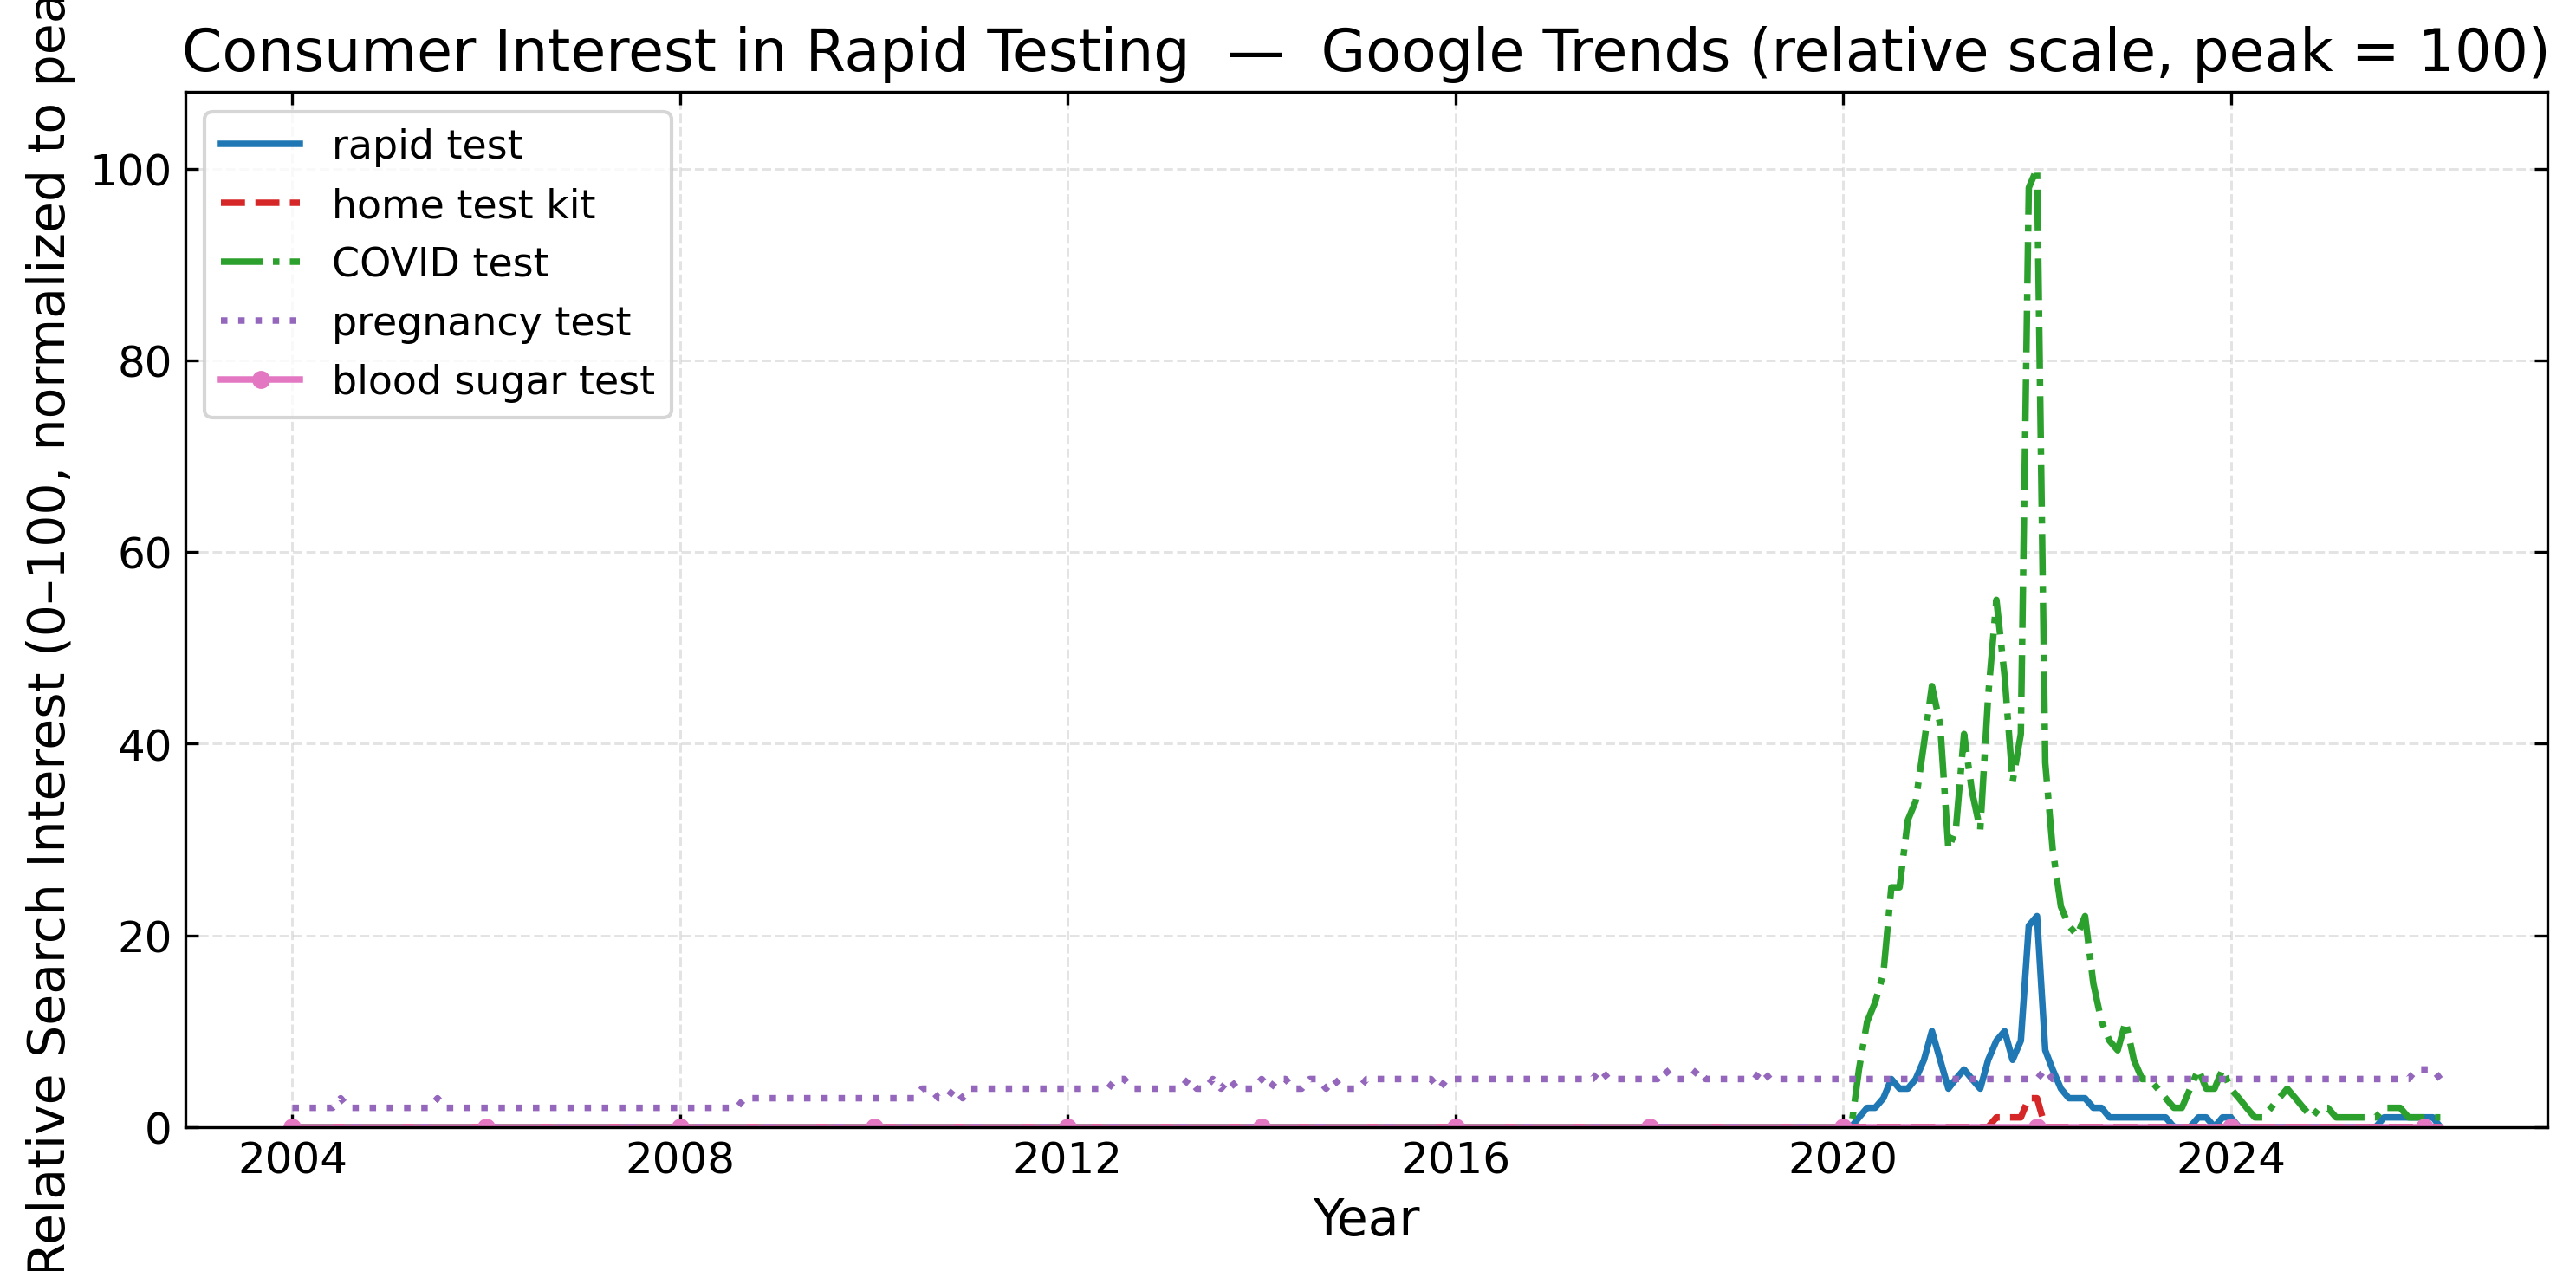
\includegraphics[width=1\linewidth]{Abbildungen/Intro/graph2_consumer_trends.png}
    \caption{Caption}
    \label{fig:placeholder} 
\end{figure}
These \ac{POCT} also come with their own limitations.
For once, the...
Additionally...
Therefore, after a first test at home, more elaborate diagnostics such as PCr... are still commonly used to get more accurate results and, therefore, allow for precise monitoring and treatment. 

-- The struggle: why we need new tests? Where do PCR and such fail, or are cumbersome or expensive?

Laboratory techniques such as the mentioned PCR, however, rely on modern infrastructure, expensive medical equipment, and trained laboratory staff, which are often limited to more developed nations with a working medical system. 
 

The search for new diagnostics is consequently highly desired and sparked a great branch of research in the last decades.
Figure \ref{fig:number_publications_POC} illustrates just that: in the last 35 years, the number of publications concerning \ac{POCT} has significantly increased, almost 18-fold, from a combined 240 publications in the field in 1990 to over 4230 publications in 2021.

\begin{figure}
    \centering
    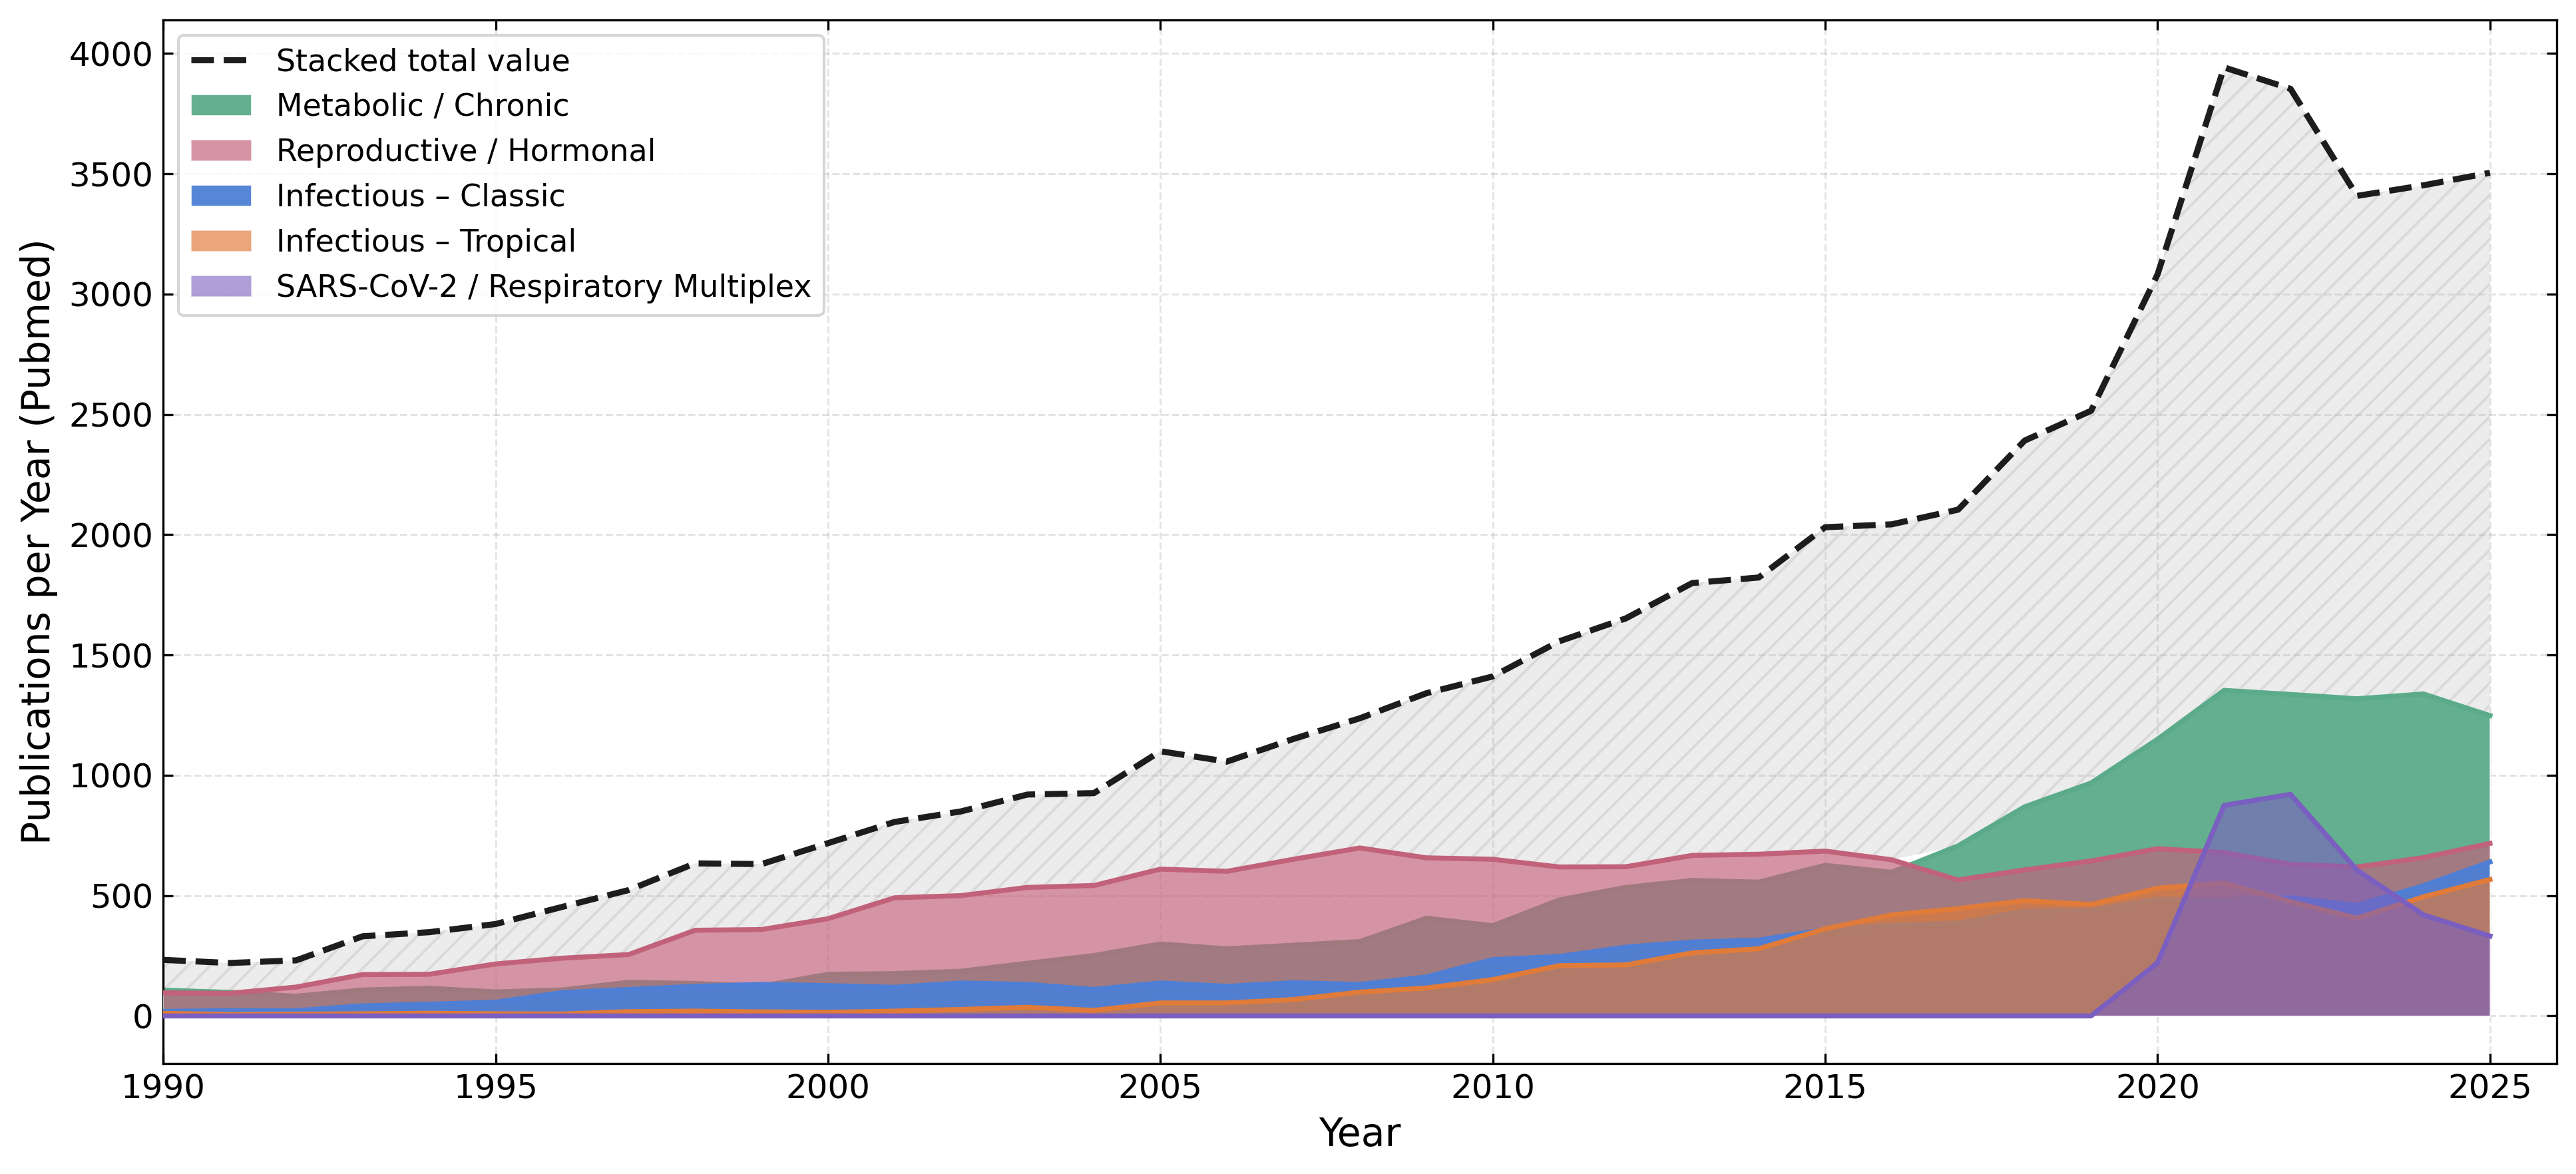
\includegraphics[width=1\linewidth]{Abbildungen/Intro/graph3_top5_categories_area_nonstacked_2025.png}
    \caption{
            Rapid test research interest by category, from 1990 to 2025 PubMed. 
            Absolute number of publications with the sum of publications shown in the dashed black area.}
    \label{fig:number_publications_POC}
\end{figure}

\ac{POCT} using magnetic particles is one emerging field. 
They are employed in so-called \ac{LOC}.
There, they promise various advantages over their paper-chromatography-based counterparts in standard \ac{POCT} devices. 
For once, the substrate, consisting of a magnetic stray field creating layer, is reusable and acts as the base of the device.
The \acp{MP}, which take up the role as the probes, are functionalized chemically on their polymer-coated surface that enables them to interact with different chemical groups. 
This means that after a given test is performed on one given device and the substrate is rinsed with water, a second test can be performed right away, allowing for many types of \acp{MP} to perform very different tests. 
As the quantity of \acp{MP} used is minute, this keeps the cost of each test low.
Different approaches using these magnetic \ac{LOC} systems are being researched. 
For the magnetic stray field creation, micromagnets are used, electrical wires for electromagnetic creation, and even...
These, however, are topographically elevated elements, limiting these devices to \ac{MP} transport far away from the substrate's surface. 
The emerging magnetic strayfield gradient needed to exert a magnetic force on the particles is washed out and not well defined, limiting the transport to... forces such as DLVO   
Topographically flat substrates, however, allow the \acp{MP} to be close to the surface, where they see a much more defined and stronger magnetic field gradient, additionally opening up the surface sensitive \ac{DLVO} forces such as electrostatic (repulsion) and van der Waals (attraction).
One method to create topographically flat magnetic substrates is the use of \ac{IBMP}, which allows for...  
\begin{figure}
    \centering
    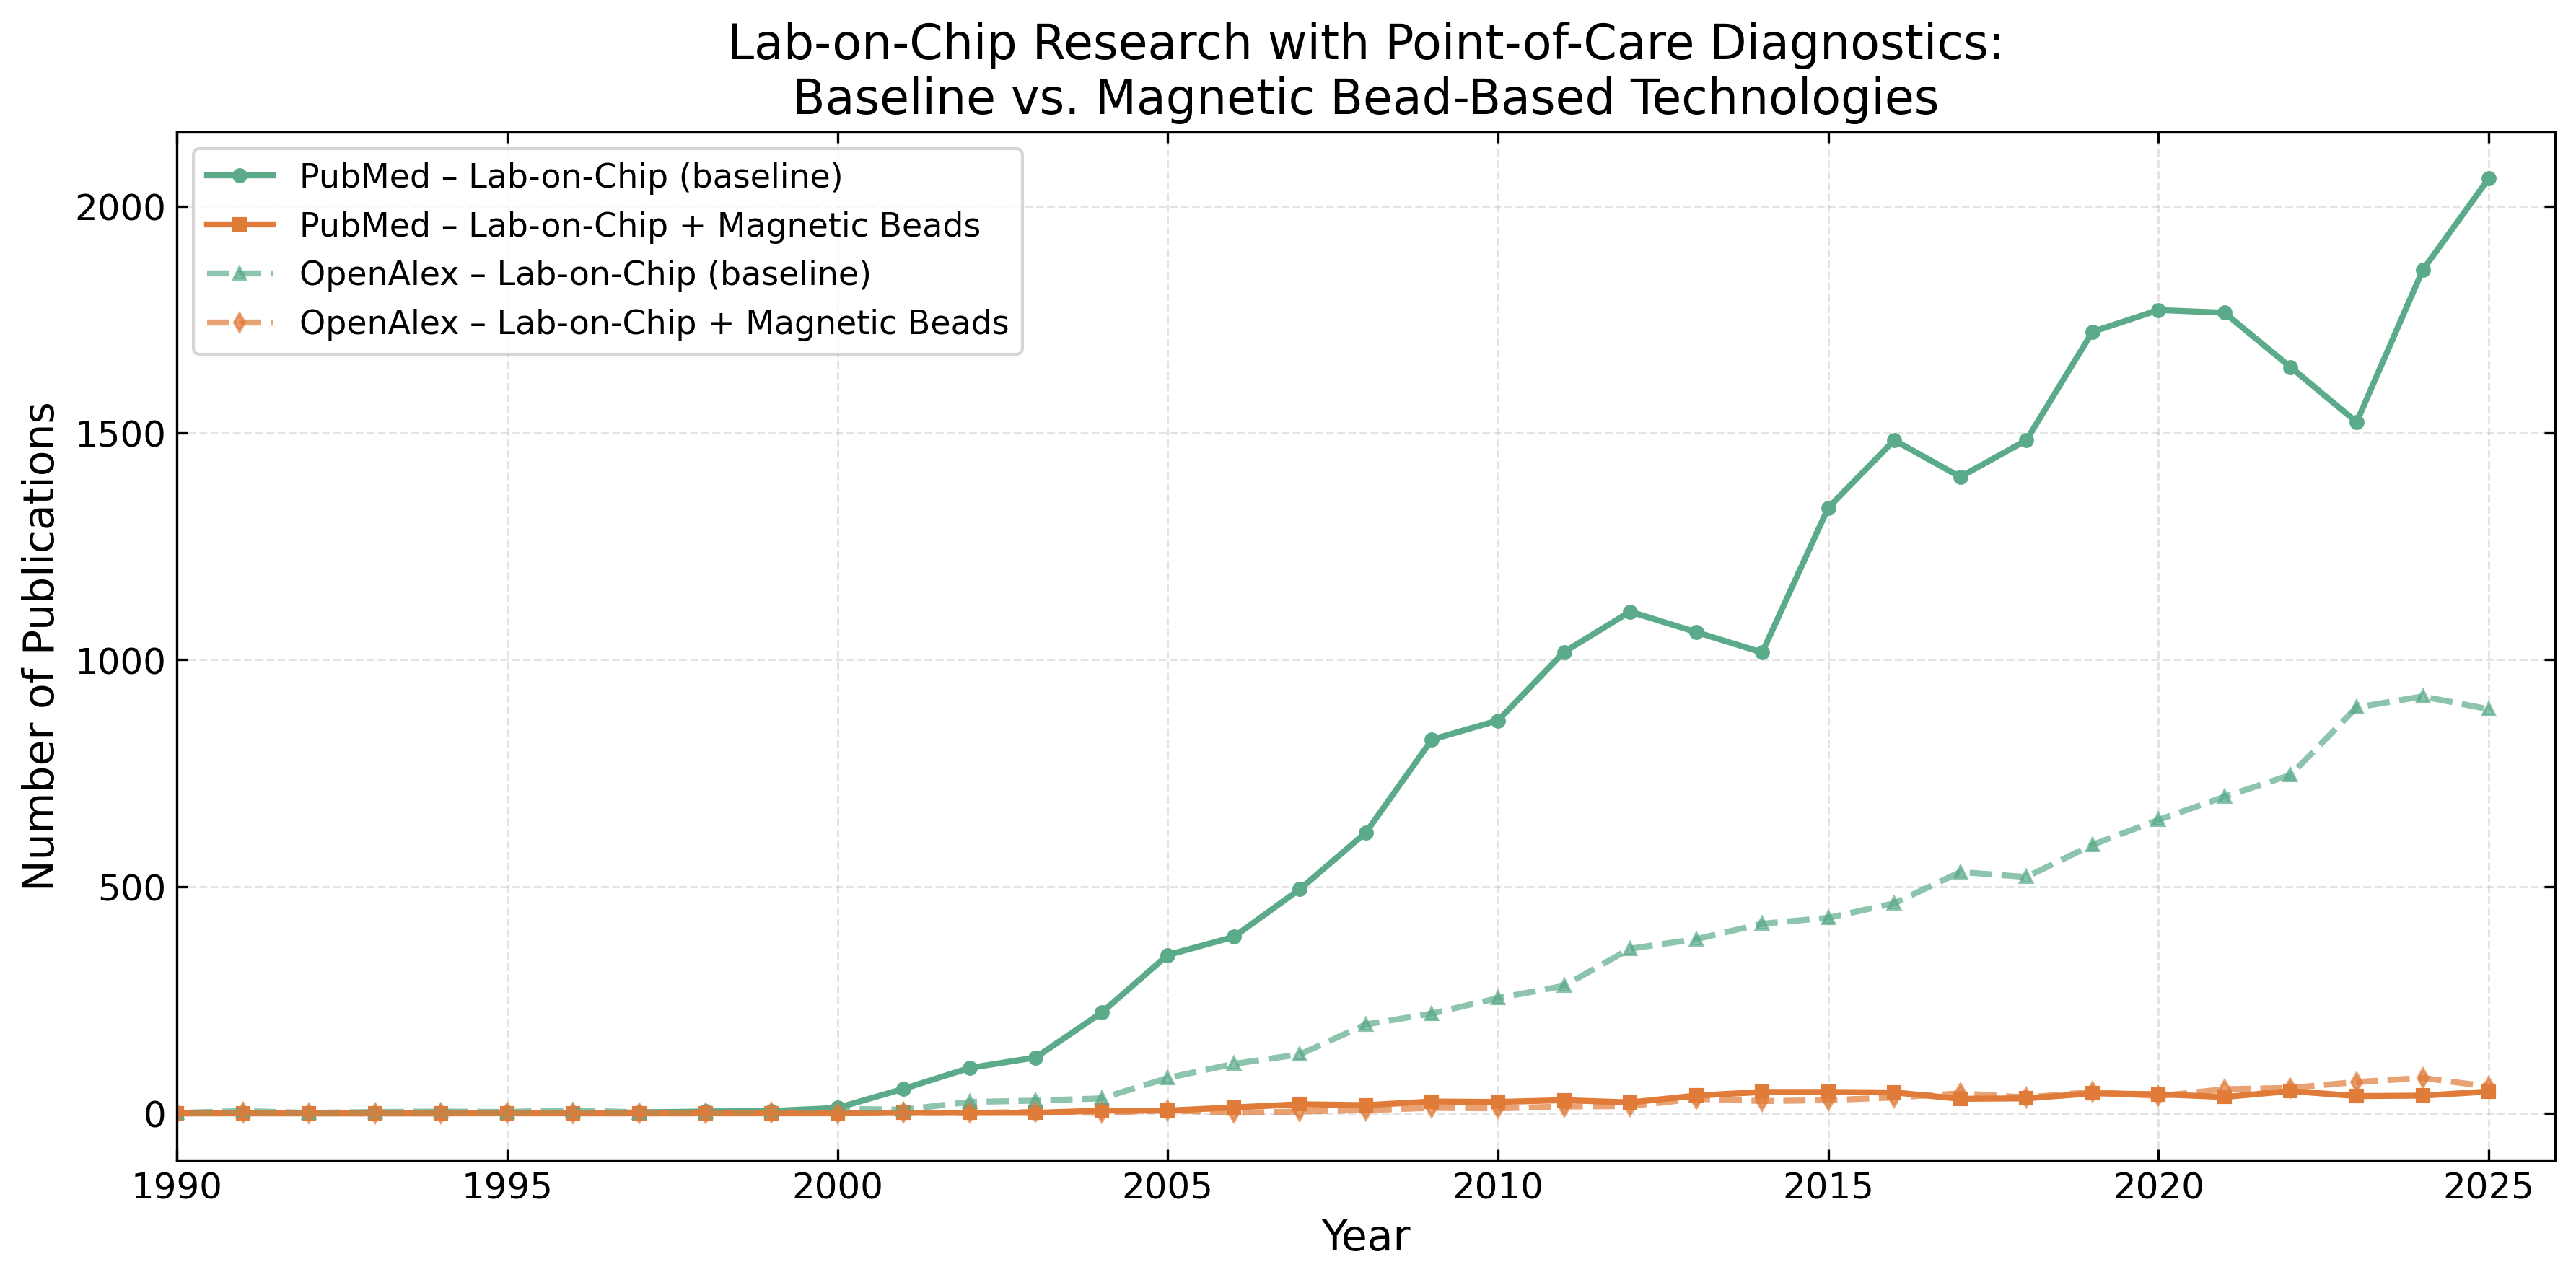
\includegraphics[width=1\linewidth]{Abbildungen/Intro/graph4_lab_on_chip.png}
    \caption{Lab on chip total research and magnetic-based Lab on chip}
    \label{fig:number_publications_lab_chip}
\end{figure}

This work focuses on the physical and chemical interactions only possible by the surface close transport of the \acp{MP} on topographically flat magnetic substrates, where the key difference in interactoin is the electrostatic repulsion that, at the distances of xxx micrometer, greatly influences the drag feeled by the \acp{MP} which, in turn, greatly change the transport dynamics of two \ac{MP} species. 
A basic sketch of this differentiation is shown in Figure \ref{fig:toc}, where the blue \acp{MP} experience a larger electrostatic repulsion due to the more pronounced negative surface charge that forms in solution by the terminal chemical groups compared to the orange \acp{MP} that, while crusually being negative as well, is mixed with chemical groups that, in solution, induce positive charges. 

\begin{figure}
    \centering
    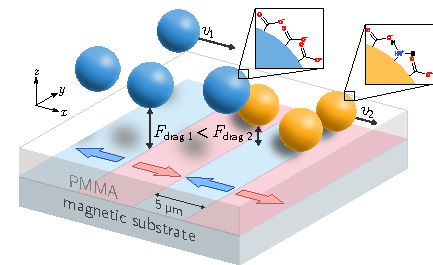
\includegraphics[width=0.8\linewidth]{Abbildungen/Drawing Board/3D-Substrate.pdf}
    \caption{
        Sketch of the relevant forces acting on the two different \acp{MP} suspended in a liquid above the prototypical \ac{EB}-coupled magnetically stripe-domain patterned transport substrate.
        The two functional groups are indicated: purely carboxylic group on the blue \acp{MP} and a mixture of carboxylic and amino group on the orange \acp{MP}.
        Since the \acp{MP} are suspended in water, a proton dissociates from the carboxylic group to form \ch{COO-} while the amino group is protonated to \ch{NH3+}.
        This is what changes the surface potential and, therefore, the Zeta potential of the \acp{MP}.
        }
    \label{fig:toc}
\end{figure}

The Figure shows the prototypical stripe domain pattern with \SI{5}{\micro\m} wide \ac{hh}/\ac{tt}-domains referring to the magnetization direction with respect to the $x$-transport-direction.
The Magnetic layer stack is discussed later, as well as the \ac{PMMA} spacing layer needed to create the repelling equal charges necessary. 
Forces along $x$ and $z$ are indicated with magnitude and direction, which then result in the also indicated velocity of the \acp{MP}. 

The first chapter of this thesis will dive into the underlying transport dynamics of the aforementioned surface close transport of two physically identical \acp{MP} of \SI{1}{\micro\m} radii containing nanoscopic magnetite, only differing in the chemical composition of the surface coating, where one species only contains carboxylic end groups \ch{COOH}, while the other mixes the \ch{COOH} groups with amino groups \ch{NH2}.
Being suspended in water at $\mathrm{pH}=7$, \ch{COOH} dissociates into \ch{COO-} while \ch{NH2} is protonated to \ch{NH3+}, which is the origin of the charge; this is depicted in Figure \ref{fig:toc} in the two zoom-ins.  

Chapter 2 will...
Chapter 3 deals with...